\chapter{Methodology}\label{ch:method}

\begin{guide}
About 8--10 pages. Describe what was \emph{done}, in enough detail that someone could rebuild it. Results do not go here. Start from the proposal's Methodology chapter and correct it wherever the implementation differs (the differences are listed in \cref{sec:deviations}).
\end{guide}

\section{Framework overview}
\begin{figure}[ht]
  \centering
  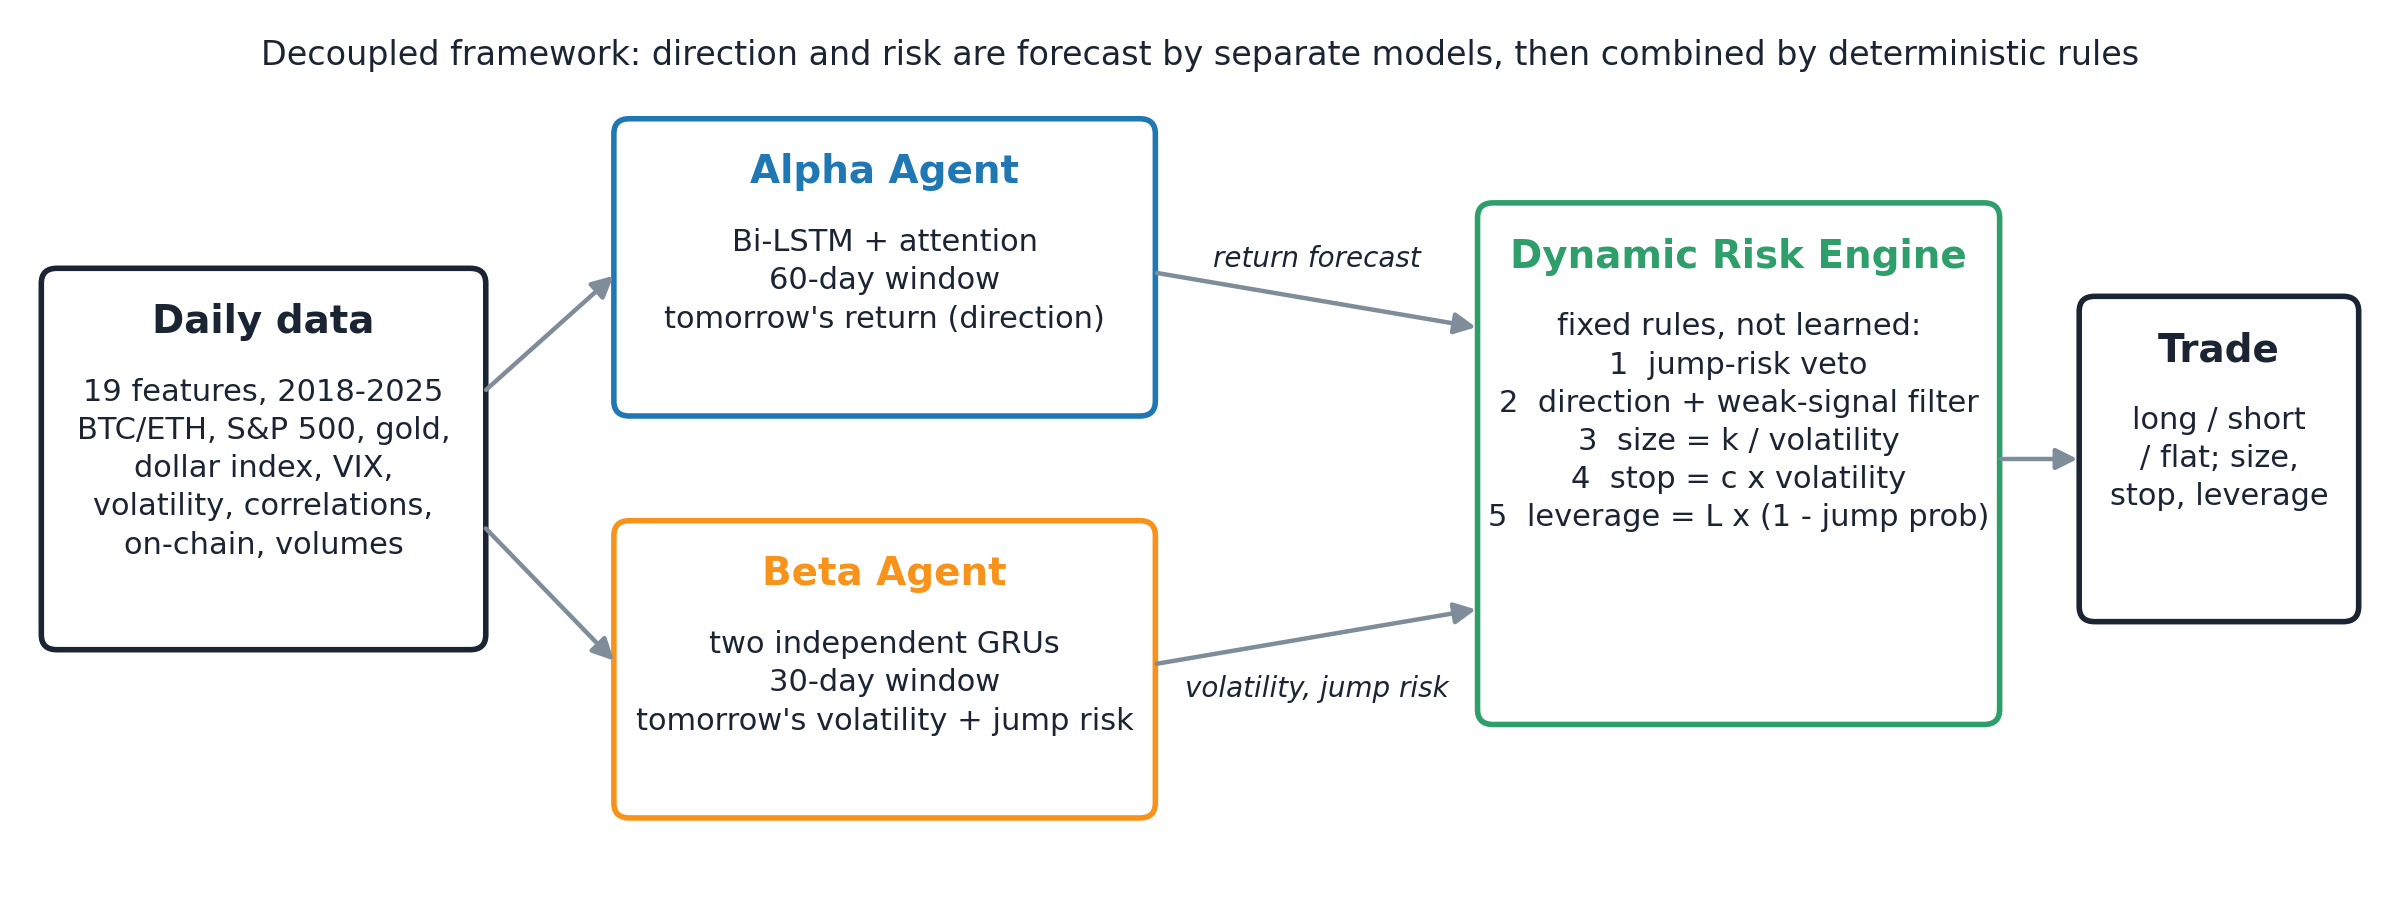
\includegraphics[width=\textwidth]{framework_diagram.png}
  \caption{The decoupled framework: direction and risk are forecast by separate models, then combined by fixed rules.}
  \label{fig:framework}
\end{figure}
\tbc{one paragraph walking through \cref{fig:framework}; explain why decoupling: each model has one job, and the risk side can work even when the direction side cannot}

\section{The Alpha Agent}
\begin{guide}
Bi-LSTM over a 60-day window of all 19 features, followed by single-head attention whose query is the last time step and whose keys/values are the whole sequence; output is $\hat r_{t+1}$. Give the attention equations (score, softmax weights, context vector). Note the implementation detail that the baseline Bi-LSTM pools with the final hidden state of each direction (\texttt{h\_n}), not the last output step, because the backward direction's last output has seen only one step.
\end{guide}
\tbc{}

\section{Baselines}
\tbc{Vanilla LSTM and GRU (univariate), Standard Bi-LSTM (multivariate, no attention), univariate Bi-LSTM for the clean H1 test, naive ``no change'' forecast; GARCH(1,1) and persistence for volatility}

\section{The Beta Agent}\label{sec:beta}
\begin{guide}
Two independent GRUs (32 units), 30-day window: one regresses $|r_{t+1}|$, one classifies jump risk. The jump probability is calibrated with Platt scaling on 2024. Explain why two separate networks rather than one with two heads (\tbc{your reason}).
\end{guide}
\tbc{}

\subsection{Choice of volatility target}\label{sec:vol-target}
\begin{guide}
Important: this is a genuine methodological finding, so give it space. The proposal's target was 14-day rolling volatility. Today's and tomorrow's 14-day windows share 13 days, and today's value was also an input, so persistence wins by construction: the model lost to it by 766\%, and five fixes (predicting the change, adding GARCH as an input, and combinations) all still lost. On the supervisor's suggestion the target became the size of the next day's move $|r_{t+1}|$, which beats persistence (\cref{sec:res-vol}). Use \texttt{phase3\_volatility\_target.png} either here or in Results - not both.
\end{guide}
\tbc{}

\section{The Dynamic Risk Engine}\label{sec:risk-engine}
\begin{guide}
Five deterministic rules - write each as an equation with its parameter:
\begin{enumerate}
  \item \textbf{Jump veto:} no trade if $\hat p_{\text{jump}} > \tau_j$.
  \item \textbf{Direction and strength filter:} long if $\hat r_{t+1} > 0$, short if $< 0$, but only if $|\hat r_{t+1}|$ is above the $\tau_y$ percentile of recent forecasts.
  \item \textbf{Volatility sizing:} position fraction $= k / \hat\sigma_{t+1}$ (capped).
  \item \textbf{Volatility stop:} stop distance $= c \cdot \hat\sigma_{t+1}$.
  \item \textbf{Jump-scaled leverage:} $L = L_{\max}(1 - \hat p_{\text{jump}})$.
\end{enumerate}
Then the \textbf{fixed-rule ablation} used for H3: same direction signal, but fixed size, fixed stop, no veto, constant leverage - i.e.\ the same system with the Beta Agent removed. State that both engines were tuned the same way.
\end{guide}
\tbc{}

\section{Training procedure}
\tbc{loss functions; Adam (lr $10^{-3}$), batch 64, early stopping after 10 epochs without validation improvement, learning rate halved after 5, gradient clipping at norm 1.0; 5 fixed seeds (0--4), results reported as mean $\pm$ std over seeds; full table in \cref{app:hyper}}

\section{Backtest design}\label{sec:backtest}
\begin{guide}
The rules of the simulation, as a list: R1{,}000 starting capital; one decision per weekday; stops and liquidation checked on every calendar day's high/low, including weekends (BTC trades 24/7); 0.1\% round-trip cost; liquidation loses the full margin; stops fill at the stop price (no slippage - a limitation). Tuning: grid search on 2024 maximising Sharpe minus max drawdown; the chosen parameters are then frozen for 2025 and 2026. Leverage cap $L_{\max} = 2$ in the main results (the EU retail cap for crypto CFDs), with 5x, 10x and 20x in a stress test.
\end{guide}
\tbc{}

\section{Evaluation}\label{sec:evaluation}
\subsection{Forecast metrics}
\tbc{RMSE (main), MAPE (for comparison with the literature), hit rate with Wilson 95\% intervals}

\subsection{Trading metrics}
\begin{guide}
Define each with a formula: final balance; max drawdown $= \max_t \big(1 - V_t / \max_{s\le t} V_s\big)$; Sharpe $= \sqrt{260}\,\bar r / s_r$ with risk-free rate 0; Sortino; number of liquidations.
\end{guide}
\tbc{}

\subsection{Statistical tests}
\begin{guide}
Diebold--Mariano tests for forecast errors (per seed). For trading results: a DM-style test on daily returns with Newey--West variance, and a paired moving-block bootstrap (5{,}000 resamples, 10-day blocks) for differences in drawdown and Sharpe, giving 95\% intervals and one-sided $p$-values. Explain in one sentence why blocks: returns are not independent day to day.
\end{guide}
\tbc{}
